\documentclass[conference]{IEEEtran}
\usepackage{mathptmx}
\usepackage{iftex}
\ifPDFTeX\else
\usepackage{fontspec}
\setmainfont{texgyretermes-regular.otf}[
BoldFont=texgyretermes-bold.otf,
ItalicFont=texgyretermes-italic.otf,
BoldItalicFont=texgyretermes-bolditalic.otf]
\fi
\usepackage{amsmath,amssymb,booktabs,graphicx,url,array}
\usepackage[hidelinks]{hyperref}
\usepackage{balance}
\graphicspath{{figures/}}
\newcommand{\R}{\mathbb{R}}
\title{When Should Experts Expand?\\Evidence from Synthetic Streams and Neural MNIST Experiments}
\author{\IEEEauthorblockN{Mingqi Li and Kaiyue Zhang}
\IEEEauthorblockA{COMPSCI 764 Research Project\\University of Auckland}}
\begin{document}
\maketitle
\thispagestyle{plain}
\pagestyle{plain}
\begin{abstract}
Dynamic expert expansion can protect incompatible updates, but input change alone may not justify new capacity. We study whether combining novelty with gradient interference reduces allocation while retaining prediction quality. A controlled synthetic study compares four policies across four streams and ten matched seeds. A real-image extension trains 109,386-parameter, two-hidden-layer networks from MNIST pixels on contrast and permutation streams with five matched seeds. A separate exploratory label-remapping stress adds conflicting targets. Five neural policies include a revision that retains unresolved novelty after routing-prototype admission. In the synthetic study, joint triggering reduces benign allocation but underperforms novelty-only under conflicting and mixed rules. On MNIST contrast, joint accuracy is 93.61\% using one expert, compared with 91.30\% using three for novelty-only. On permutation, the corresponding accuracies are 91.95\% and 92.00\%. However, fixed capacity matches joint predictions, and retained evidence produces no additional improvement. Joint control reduces recorded neural storage by approximately 28--30\% while processing about 25\% more gradient examples. These results distinguish selective allocation from evidence that adaptive growth is necessary. They support a bounded mechanism study, while leaving harder datasets, learned routing and large-model experts unvalidated.
\end{abstract}
\begin{IEEEkeywords}
continual learning, expert expansion, gradient interference, novelty detection, controlled experiments
\end{IEEEkeywords}
\section{Introduction}
\subsection{Problem and motivation}
Continual learning requires a predictor to adapt to incoming observations while retaining useful earlier knowledge. Neural updates can improve recent examples and damage historical ones. Architectural expansion addresses this tension by adding components that specialize while preserving established parameters. Progressive Neural Networks protect earlier columns and transfer through lateral connections \cite{pnn}. Expert Gate introduces input-dependent selection among specialists \cite{expertgate}. These approaches make the allocation and selection of capacity part of learning.

The number of encountered domains need not equal the number of predictive functions required. Changed lighting or intensity can preserve a label's meaning, several contexts can share one rule, and earlier contexts can recur. Conversely, incompatible rules can require separation even when a distribution detector sees little change. Allocating a new network whenever input looks unfamiliar may waste capacity. Reusing a network whenever context looks familiar can also miss an unresolved predictive mismatch.

Our literature review originally proposed expansion, routing, merging, pruning and distillation within one lifecycle. The present project narrows this scope to the expansion decision. It does not implement the complete lifecycle, pretrained backbones or adapters. This restriction makes a specific hypothesis testable: whether input novelty combined with historical gradient risk is a better allocation signal than novelty alone. We examine complete controllers, including their routing state and memory, because the meaning of a score can change when those states change.

\subsection{Research questions and hypotheses}
The primary question is: \emph{Compared with novelty-only allocation, can a joint novelty--interference trigger use fewer experts while maintaining final accuracy?} The hypothesis is that compatible changes should permit reuse, while sustained novel and incompatible updates can justify specialization. Capacity reduction alone is insufficient evidence if it arises from missing a new rule.

The two signals have different interpretations. Novelty measures distance from stored context prototypes. Gradient interference measures local opposition between current and historical data gradients, motivated by GEM and A-GEM \cite{gem,agem}. Their conjunction is conservative: either weak signal prevents allocation. Conservatism can suppress redundant growth, but persistence requirements can delay useful specialization. A prototype can even make unfamiliar input appear familiar before enough consecutive conflict observations accumulate.

This motivates a secondary question: \emph{Does temporarily retaining unresolved novelty after prototype admission improve the joint controller?} We implement a retained-evidence variant for the neural extension. Its acceptance rule, lifetime and evaluation are explicit. We do not assume that identifying a plausible timing problem guarantees an improved algorithm.

\subsection{Two levels of evidence}
The first study uses synthetic binary streams and three-parameter logistic experts. Its supplied separation between predictive and contextual coordinates permits a transparent analysis of conflicting rules, recurrence and ambiguous routing. It is a mechanism experiment, not a deep-network benchmark.

The second study trains two-hidden-layer neural experts directly from real MNIST images \cite{mnist}. Each expert has 109,386 learned parameters. Raw image pixels serve both the classifier and the input-prototype router; no extra context coordinates are supplied. Contrast and pixel-permutation streams test sharing and changed input representations. A separately documented exploratory stress also remaps target labels. These are constructed streams derived from real images, rather than reproductions of published continual-learning benchmark protocols.

Neither learner receives domain identifiers or segment boundaries. The evaluator alone uses this information. Homogeneous training windows, a fixed warm-up prefix and short scripted sequences nevertheless simplify the problem. These assumptions and the limited number of seeds constrain generalization.

\subsection{Contributions and outcome}
The project provides a bounded, reproducible comparison with explicit information access, matched data and resource accounting. It diagnoses a coupling between novelty evidence and prototype admission, then tests a concrete retained-evidence revision with learned neural features. It also distinguishes weight-array savings from total retained-array storage and the additional work required to compute interference.

The outcome remains conditional. Joint gating suppresses redundant allocation, but fails on some conflicting synthetic streams. In the neural experiments it often follows exactly the fixed-capacity trajectory. The retained revision makes more windows eligible for joint decisions, yet does not produce additional allocations or accuracy gains. Thus the evidence supports selective reuse in these settings, not general superiority over a fixed network or a validated large-model lifecycle.

\section{Related Work}
Progressive Neural Networks protect past columns and transfer through lateral connections \cite{pnn}. Expert Gate uses reconstruction-based task models to route inputs among specialists \cite{expertgate}. Their distinction between isolation and selection motivates our explicit router, but neither full system is reproduced. Our raw-pixel nearest-prototype selector is substantially simpler than learned gating.

DEN selectively retrains, expands and splits units \cite{den}. Learn to Grow separates neural structural choices from parameter learning, permitting reuse, adaptation or new structure \cite{l2g}. These approaches show why a declared task need not imply copying an entire network. Our comparison fixes expert architecture and isolates a binary allocation decision. Learn to Grow also evaluates permuted MNIST, but our short, recurring streams, smaller data budget and task-free routing differ from its published protocol; scores are not directly compared.

GEM constrains updates using episodic memories \cite{gem}. A-GEM uses an averaged historical gradient and emphasizes evaluation with disjoint hyperparameter-selection tasks \cite{agem}. Their first-order interpretation motivates our interference score. We do not perform their gradient projection or claim their retention guarantees. A negative cosine is a diagnostic risk estimate, not measured forgetting or proof that another expert is needed.

DER expands representations and prunes redundancy \cite{der}; FOSTER combines expansion with feature boosting and compression \cite{foster}. MEMO considers model storage together with exemplars and shares general features while extending specialized ones \cite{memo}. These works motivate resource accounting beyond expert count. Their class-incremental image architectures and label-space protocols differ from this study's fixed ten-class neural tasks and controlled binary rules.

MoE adapters attach lightweight experts to a pretrained vision-language model \cite{moeadapters}. Lightweight experts still require an allocation policy, but our networks learn from MNIST pixels without a pretrained backbone. We test a trigger hypothesis related to these systems, rather than a replacement for their architectures. The retained-evidence variant changes when novelty remains available to that trigger; it does not add merging, distillation or an independently learned router.

\section{Methodology}
Code and recorded experimental results are provided in the project repository.\footnote{\url{https://github.com/jdjhc/compsci764-expert-expansion}. The repository is publicly accessible.}
\subsection{Setting and information access}
At window \(t\), the learner receives a batch \(B_t\) of observations, labels and chronological identifiers. It maintains a bank of experts, a bounded input-prototype gallery and a bounded historical reservoir. Segment identifiers, transformation parameters and domain labels are withheld. The evaluator uses them only to construct streams, log outcomes and measure per-domain accuracy.

In the synthetic study each observation contains predictive coordinates \(x\in\R^2\) and separate context \(c\in\R^2\). Classification uses \(x\), while routing uses \(c\). In the neural study the normalized image \(x\in[0,1]^{784}\) supplies both roles. No manufactured context coordinate is appended. Training chooses one candidate from the current batch mean; test-time routing operates on each individual image. Homogeneous batches therefore provide an easier training context than arbitrary mixtures within a window.

Decisions use strictly earlier reservoir entries. Current examples enter memory only after optimization. An assertion checks that all cached chronological identifiers precede the current window. The synthetic interfaces additionally reject negative test identifiers; neural testing uses a separate evaluator interface. Formal MNIST stream indices exclude every image used in development or threshold calibration and all official test images.

\subsection{Expert models}
A synthetic expert has \(\theta_e=(w_{e,1},w_{e,2},a_e)\) and probability
\begin{equation}
p_e(y=1\mid x)=\sigma(w_e^\top x+a_e).
\end{equation}
It uses mean binary cross-entropy. For residual \(r_i=p_e(x_i)-y_i\), its data gradient is
\begin{equation}
g_e(B)=|B|^{-1}\begin{bmatrix}\sum_i r_ix_i\\\sum_i r_i\end{bmatrix}.
\end{equation}
The first expert starts at zero. New experts clone the candidate's parameters.

A neural expert is a multilayer perceptron:
\begin{align}
h_1&=\operatorname{ReLU}(xW_1+b_1),\\
h_2&=\operatorname{ReLU}(h_1W_2+b_2),\\
p_e(y\mid x)&=\operatorname{softmax}(h_2W_3+b_3),
\end{align}
with dimensions \(784\!\rightarrow\!128\!\rightarrow\!64\!\rightarrow\!10\). There are 109,386 trainable parameters: 100,480 in the first affine layer, 8,256 in the second and 650 in the output. Two hidden layers learn features directly from pixels. This is a small deep-learning experiment, not a pretrained vision model.

Weights use independent zero-mean normal initialization with variance \(2/d_{\mathrm{in}}\); biases start at zero. Neural data loss is mean ten-class cross-entropy, evaluated with shifted logits for numerical stability. Parameters, activations and updates use float32. Forward and reverse computations are implemented in NumPy. Finite differences check all parameters of a small network with the same three-layer computational structure. Full experts are copied on expansion; there is no momentum or optimizer state to reset.

\subsection{Optimization and historical replay}
Each window performs four SGD steps. When eligible history exists, the data gradient is
\begin{equation}
g_{\mathrm{train}}=(1-\lambda)g_{\mathrm{current}}+\lambda g_{\mathrm{replay}},\qquad\lambda=0.25.
\end{equation}
Each step independently draws a replay batch uniformly among cached examples currently routed to the selected expert. Sampling is without replacement when enough examples exist and with replacement otherwise. Without eligible history, the current gradient receives full weight. Weight decay adds \(10^{-4}W\) to weight gradients; biases are unregularized. The learning rate is 0.15 for logistic experts and 0.1 for neural experts.

Only the selected expert is updated. New experts initially inherit earlier features and can adapt them; old experts retain their parameters. However, changed routing can make an old expert unreachable or change the history eligible for another expert. Equal optimizer rules and reservoir sizes consequently do not imply equal realized replay or computation. Four reuses of the current batch also mean this is a windowed streaming protocol, rather than strict one-pass example-level learning.

\subsection{Routing and novelty}
The gallery stores anchors \(\mu_j\) and expert assignments \(q_j\). For context representation \(z\),
\begin{equation}
j^*(z)=\arg\min_j\|z-\mu_j\|_2,\qquad e(z)=q_{j^*(z)}.
\end{equation}
The first window initializes one anchor at its mean, assigned to expert zero. Training selects a candidate using current mean \(\bar z_t\), and novelty is
\begin{equation}
N_t=\min_j\|\bar z_t-\mu_j\|_2.
\end{equation}
Recognized input updates its nearest anchor as \(0.95\mu_j+0.05\bar z_t\). Novel means enter a three-entry buffer. Three consecutive novel windows can admit their mean as another anchor, even without expansion. This allows several contexts to share an expert. The buffer requires novelty, not a supervised declaration that all entries share one task. Rapid alternating changes could therefore produce a poor prototype and are outside the tested homogeneous streams.

A novel expert immediately receives its own anchor, preserving old assignments. Expansion at a recognized context reassigns the nearest anchor. An expert without any remaining assignment still counts toward storage. The gallery cap is twelve. Novel creation requires a free gallery slot so that the newly created specialist is reachable.

Both novelty thresholds are independently calibrated at a 99.5th percentile of 512 pairs of stationary batch means. Synthetic calibration uses known Gaussian noise and independent seed 20261024, giving 0.2419615681. Neural calibration uses only raw training images 0--1999, no labels, and the same independent calibration seed. Sampling two batches of 100 images with replacement gives threshold 1.4203898907. It calibrates the original-image domain, not every contrast or permutation distribution. Neither threshold is fitted against held-out accuracy.

\subsection{Gradient interference}
Let \(g_t\) be the candidate's current data gradient and \(g_M\) its data gradient on eligible earlier memory. The score is
\begin{equation}
I_t=\max\left(0,-\frac{\langle g_t,g_M\rangle}{\|g_t\|_2\|g_M\|_2}\right).
\end{equation}
For a neural expert, inner products sum over every weight and bias array. Reference data are the deterministic prefix of up to 64 eligible entries in the current priority-reservoir array; this is not a new random reference sample at each window. Eligibility is recomputed under current routing. A small gradient norm makes the score zero and unreliable, using floors \(10^{-6}\) for synthetic and \(10^{-8}\) for neural calculations. Without eligible history, the condition is false. The interference threshold is 0.2.

For a current-only step \(\theta'=\theta-\eta g_t\),
\begin{equation}
L_M(\theta')-L_M(\theta)\approx-\eta\langle g_M,g_t\rangle.
\end{equation}
Opposition motivates concern about increasing historical loss. The actual optimizer mixes replay, regularization and multiple steps, so the approximation does not exactly predict its update. Gradient cancellation, incomplete memory, curvature and small residuals can all weaken the signal. Normalizing also discards magnitude: small opposing gradients can yield a large score. These limitations motivate explicit evaluation instead of treating conflict as a certificate of insufficient capacity.

\subsection{Policies, persistence and retained evidence}
Fixed capacity never expands. Novelty requires \(N_t>\tau_N\); Interference requires \(I_t>0.2\); Dual requires both. The primary rule needs three consecutive qualifying windows with the same existing candidate. A false condition or changed candidate resets the streak. Allocation is disabled during the fixed warm-up and constrained by a three-window cooldown and four-expert cap. A completed streak at capacity records a blocked request and reuses the candidate.

The retained variant changes only the availability of novelty evidence. If a novel context is admitted without expansion at window \(u\), that anchor receives unresolved status through \(u+30\). When input matches it, the gate uses
\begin{equation}
\widetilde N_t=\mathbf{1}[N_t>\tau_N]\ \lor\ \mathbf{1}[t\leq\mathrm{expiry}(j^*)].
\end{equation}
The expansion condition becomes \(\widetilde N_t\land(I_t>0.2)\), with the same candidate-specific consecutive streak. Successful expansion clears the relevant status; expiry also ends its effect. Ordinary prototype averaging does not clear it. The 30-window lifetime is a specified diagnostic setting, not an optimum. Retention can admit noisy later conflicts and create unnecessary experts, and it cannot help when conflict never persists for three windows.

\subsection{Update order and bounded state}
At each window the controller: (1) selects the old candidate and measures novelty; (2) computes required gradients from past memory; (3) updates the streak and allocates if permitted; (4) admits or updates gallery state; (5) recomputes replay eligibility and optimizes the selected expert; and (6) inserts current examples into the reservoir. The retained policy intervenes at the gate; it does not freeze the model during an unresolved change.

Each arriving example receives an independent uniform priority; the reservoir retains the largest priorities up to its cap. Shared priorities make global historical contents identical across policies, while routing may change eligible subsets. For gallery size \(m\), context dimension \(d\), memory size \(M\) and expert size \(q\), routing is \(O(md)\) per example. Reference and replay operations also route cached examples. State is bounded by four experts, twelve anchors, one bounded reservoir and three pending means. Bounds do not establish adequacy: exhausted slots or unreachable experts can still prevent useful specialization.


\section{Experimental Protocol}
\subsection{Synthetic mechanism study}
Predictive input follows \(x\sim\mathcal N(0,I_2)\), independently of context \(c\sim\mathcal N(\mu_d,0.45^2I_2)\). Domain \(d\) labels by \(\mathbf{1}[v_d^\top x\geq0]\), then flips each label independently with probability 0.05. The best population accuracy with the correct rule is approximately 95\%.

Benign shifts use contexts \((0,0),(5,0),(0,5)\) and one rule \((1,0.6)\), in order A,B,C,A,B,C. Conflicting shifts keep those contexts and order but use rules \((1,0.6),(-1,-0.6),(0.6,-1)\). Mixed recurrence uses four contexts \((0,0),(5,0),(0,5),(0,10)\), with A/B sharing the first rule and C/D its opposite, in order A,B,C,D,A,B,C,D. Hidden reversal uses identical contexts and opposite rules, in order A,B,A,B,A,B. A fixed input-only router cannot determine which opposite concept generated an observation; their balanced expected accuracy is 50\%.

Each segment has 24 windows of 64 examples. The first 24 windows are a fixed warm-up. Replay stores 256 observations, and each optimizer step draws 32 eligible examples. Each unique domain has 1,024 held-out examples per seed. Seeds 0--9 define ten matched streams, yielding 160 primary runs across four policies and four scenarios. The three earlier sensitivity configurations use persistence one or interference thresholds zero and 0.4, producing 480 additional configuration runs. They are exploratory analyses prompted by primary behavior; only corrected canonical runs are used.

\subsection{Real-image neural extension}
MNIST contains 60,000 training and 10,000 test images of handwritten digits \cite{mnist}. We preserve the official split and divide training positions further: 0--9999 are development-only, while 10000--59999 supply formal streams. Independent development trains on 6,000 images sampled from the first 8,000 and validates on positions 8000--9999. Its 89.8\% accuracy establishes a basic learnability check, not a final test result. Calibration uses unlabeled positions 0--1999 within the development partition.

For each formal seed, a permutation of the 50,000-image training pool supplies six disjoint chunks of 6,000. Every stream therefore contains 36,000 distinct source training images, 360 windows and no within-run image repetition. Domain recurrence uses new source images with the same transformation. Cross-seed training subsets can overlap; seeds are replications of a constructed task, not independent datasets.

Contrast uses A:\(x\), B:\(0.55x\), and C:\(0.55x+0.25\), preserving labels and order A,B,C,A,B,C. This tests shared semantic labels under intensity changes. It does not assert that the exact decision function is unchanged in pixel coordinates. Permutation uses identity and two fixed, seed-specific permutations of 784 pixel positions, with labels unchanged and the same recurrence order. Both networks and router receive only the transformed pixels.

Each domain is evaluated on all 10,000 official test images with its corresponding transformation. No test image or label enters calibration, replay or optimization. Test images are reused across domain transformations, policies, endpoints and seeds, so the resulting measurements are dependent. These short recurring streams differ from conventional published Permuted-MNIST protocols in data budget, sequence, architecture and access to task information.

Five matched seeds 0--4 compare Fixed, Novelty, Interference, Dual and Retained, giving 50 runs. Network initialization, training examples, transformations, test images and reservoir priorities are matched within each scenario/seed. The two-stream protocol was written before loading official test arrays. It was motivated by earlier synthetic results and is not an external preregistration. Learning rate, thresholds, lifetime and seeds were not selected using formal test accuracy.

\begin{table}[t]
\caption{Neural extension settings; differences from synthetic settings are explicit in the text.}
\label{tab:settings}\centering\small
\begin{tabular}{lr}\toprule Setting & Value\\\midrule
Network & 784--128--64--10\\
Trainable parameters per expert & 109,386\\
Examples per window / segment & 100 / 6,000\\
Optimizer steps / learning rate & 4 / 0.1\\
Replay capacity / batch & 512 / 64\\
Reference batch (maximum) & 64\\
Expert / prototype caps & 4 / 12\\
Trigger / gallery persistence & 3 / 3 windows\\
Cooldown / warm-up & 3 / 60 windows\\
Retained-evidence lifetime & 30 windows\\
Interference / novelty thresholds & 0.2 / 1.42039\\
Held-out images per domain & 10,000\\
Matched seeds & 5\\\bottomrule\end{tabular}
\end{table}

\begin{figure*}[t]\centering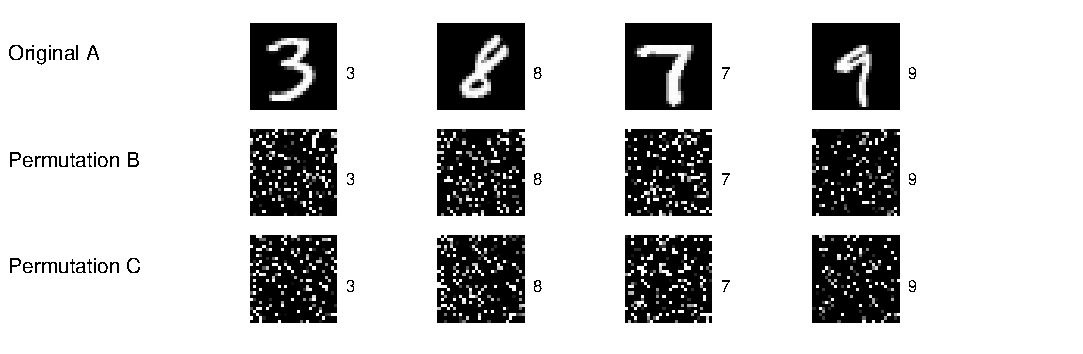
\includegraphics[width=\textwidth]{mnist_examples.pdf}
\caption{Actual MNIST training images under the seed-zero pixel transformations. Numbers beside images are original digit labels, retained in the initial permutation stream; the additional stress remaps them by domain. These examples are not generated images.}
\label{fig:mnist}\end{figure*}

\subsection{Additional conflict stress}
After the two-stream neural experiment started, we documented a separate exploratory stress. It retains the pixel permutations but changes domain labels to \((y+3d)\bmod10\), for \(d=0,1,2\). All other settings, images and seeds remain unchanged, adding 25 runs. This deliberately changes target meaning and is not ordinary digit recognition. Different permutations still supply information that can distinguish the domains, so one sufficiently expressive network can in principle fit all three mappings.

The stress is reported alongside every policy, with its post-start design status explicit. It is not an independent dataset confirmation, because it shares MNIST images and the same model family. No threshold or learning-rate search follows its test outcomes. A transformation that creates incompatible target mappings also need not create a sustained negative gradient streak in a flexible network; the logged score tests this assumption directly.

\subsection{Metrics and descriptive uncertainty}
After each segment, the evaluator tests all unique domains observed so far. Final accuracy is their unweighted mean, without increasing a domain's weight when it recurs:
\begin{equation}
A_T=D^{-1}\sum_{d=1}^D a_{T,d}.
\end{equation}
Forgetting uses endpoints after a domain first appears:
\begin{equation}
F_T=D^{-1}\sum_d\left(\max_{j\in J_d}a_{j,d}-a_{T,d}\right),
\end{equation}
where \(J_d\) includes the final endpoint. It is nonnegative but can miss within-segment failures. We also record experts, blocked requests, prototypes, gradient-sample appearances, retained-array bytes and CPU learner time. Allocated counts include unreachable experts; inference selects one network.

Tables give means and sample standard deviations. Matched seed differences use percentile bootstrap intervals: 5,000 resamples for synthetic and 10,000 for neural comparisons. They are descriptive, uncorrected for multiple comparisons and limited by ten or five independent seed pairs. The neural protocol specifies a one-percentage-point accuracy tolerance for a favorable descriptive accuracy--capacity comparison: the difference interval's lower endpoint must be above -1 point and mean allocation must decrease. This new criterion is not retroactively applied to synthetic results and is not a formal noninferiority proof.

\subsection{Implementation, checks and provenance}
Both studies use Python 3.12.14 and NumPy 2.3.5 on CPU. Neural matrix operations use one OpenBLAS thread. No PyTorch, GPU training, pretrained weights or downloaded learned representation is used. Raw MNIST archives are fetched from the mirror used by torchvision, checked against its four published MD5 values, and retained with SHA-256 provenance.

Nine synthetic checks cover gradients, historical isolation, test rejection, memory, budgets and routing assumptions. Eight neural checks additionally validate all three affine-layer gradients on a small model, parameter counts, clone independence, priority sampling, early allocation, disjoint source-image streams and a controlled delayed-conflict sequence. In that controlled sequence, retaining evidence permits a late expansion that the original conjunction misses. This verifies the implemented decision rule; it does not demonstrate a neural accuracy gain.

A previous synthetic bug overwrote old routing under early novel allocation. Corrected canonical runs preserve old anchors; archived pre-fix runs are excluded. The corrected source is shared across the four synthetic configurations. The neural source is separate and preserved exactly in both neural result directories.

The neural audit recomputes final accuracy and forgetting from raw endpoint records, checks matching hashes, source-index separation and caps, and reloads one checkpoint per policy/scenario. All fifteen reloaded models reproduce their stored final held-out accuracy. Checkpoints contain inference parameters and routing anchors, not the reservoir and RNG state required to resume optimization. Local code, protocols, manifests, raw logs and model files accompany this working project; no public repository is claimed. A real accessible repository link should replace local availability before a reproducibility-oriented public release.


\section{Results}
\begin{table*}[t]
\caption{Synthetic primary results over ten matched seeds. Accuracy is percent; forgetting is percentage points. Values show mean $\pm$ sample SD.}
\label{tab:synthetic}
\centering\small
\begin{tabular}{llrrr}\toprule Scenario & Policy & Accuracy (\%) & Experts & Forgetting (pp)\\\midrule
Benign & Fixed & 94.29 $\pm$ 0.61 & 1.00 $\pm$ 0.00 & 0.42 $\pm$ 0.29 \\
Benign & Novelty & 94.09 $\pm$ 0.48 & 3.00 $\pm$ 0.00 & 0.19 $\pm$ 0.11 \\
Benign & Interference & 94.20 $\pm$ 0.54 & 3.10 $\pm$ 1.29 & 0.42 $\pm$ 0.27 \\
Benign & Dual & 94.29 $\pm$ 0.61 & 1.10 $\pm$ 0.32 & 0.42 $\pm$ 0.28 \\
\midrule
Conflicting & Fixed & 64.31 $\pm$ 0.69 & 1.00 $\pm$ 0.00 & 29.25 $\pm$ 0.74 \\
Conflicting & Novelty & 94.07 $\pm$ 0.50 & 3.00 $\pm$ 0.00 & 0.11 $\pm$ 0.15 \\
Conflicting & Interference & 94.01 $\pm$ 0.49 & 3.30 $\pm$ 0.48 & 0.15 $\pm$ 0.15 \\
Conflicting & Dual & 89.56 $\pm$ 10.04 & 2.70 $\pm$ 0.67 & 4.34 $\pm$ 9.91 \\
\midrule
Mixed & Fixed & 49.77 $\pm$ 0.35 & 1.00 $\pm$ 0.00 & 44.50 $\pm$ 0.42 \\
Mixed & Novelty & 93.91 $\pm$ 0.45 & 4.00 $\pm$ 0.00 & 0.31 $\pm$ 0.22 \\
Mixed & Interference & 94.09 $\pm$ 0.42 & 3.40 $\pm$ 0.70 & 0.47 $\pm$ 0.26 \\
Mixed & Dual & 81.03 $\pm$ 21.02 & 2.00 $\pm$ 0.00 & 13.47 $\pm$ 20.97 \\
\midrule
Hidden reversal & Fixed & 50.00 $\pm$ 0.42 & 1.00 $\pm$ 0.00 & 44.28 $\pm$ 0.82 \\
Hidden reversal & Novelty & 50.00 $\pm$ 0.42 & 1.00 $\pm$ 0.00 & 44.28 $\pm$ 0.82 \\
Hidden reversal & Interference & 50.00 $\pm$ 0.42 & 4.00 $\pm$ 0.00 & 44.28 $\pm$ 0.82 \\
Hidden reversal & Dual & 50.00 $\pm$ 0.42 & 1.00 $\pm$ 0.00 & 44.28 $\pm$ 0.82 \\
\bottomrule
\end{tabular}
\end{table*}

\subsection{Synthetic selectivity and missed learning}
Under benign synthetic shifts, Novelty allocates three experts at \(94.09\pm0.48\%\), while Dual allocates \(1.10\pm0.32\) at \(94.29\pm0.61\%\). This suppresses redundant allocation when contexts share one rule. Fixed capacity already matches Dual accuracy with one expert, so the outcome does not establish a need for adaptive control. Interference alone allocates \(3.10\pm1.29\) despite the shared rule, showing that local gradient opposition can arise without a new predictive function being necessary.

On conflicting rules, Novelty reaches \(94.07\pm0.50\%\) with three experts; Dual reaches \(89.56\pm10.04\%\) with \(2.70\pm0.67\). Its mean forgetting is 4.34 points, compared with 0.11 for Novelty. The paired accuracy difference is -4.50 points, with descriptive interval [-12.09,0.00]. Lower allocation partly reflects missed learning. The broad interval is not evidence that the methods preserve equivalent accuracy.

Mixed recurrence makes the distinction clearer: Novelty reaches \(93.91\pm0.45\%\) with four experts, while Dual uses two but reaches \(81.03\pm21.02\%\), with 13.47 points of forgetting. Two clean rules could be represented by two specialists, yet the controller does not consistently discover and preserve that decomposition. Interference-only succeeds at \(94.09\pm0.42\%\) while using \(3.40\pm0.70\) experts. No trigger dominates accuracy, allocation and cost across every synthetic setting.

All policies approach 50\% under hidden reversal. Identical observable context cannot identify which opposite rule applies. For the same input and opposite clean binary labels, any deterministic prediction is correct for exactly one rule; equal weighting yields one half. Symmetric independent noise preserves that population bound. Interference-only nevertheless fills four slots and averages 26.3 blocked requests. Capacity detects neither a missing identifier nor an appropriate inference distinction by itself.

\subsection{Prototype admission can remove trigger evidence}
In the primary Dual logs, three of twenty novel-context admissions on conflicting streams occur without expansion, across two seeds; twenty of thirty do so under mixed recurrence. Some are appropriate when rules are shared. Admission alone is therefore not a failure label. The relevant mechanism is that the gallery needs three novel windows while the expansion gate needs three consecutive joint windows with a stable candidate.

Table~\ref{tab:trace} shows an illustrative conflicting seed. At window 24 novelty and conflict are high, but interference falls below threshold at windows 25--26. The gallery admits context at 26. Later conflict exceeds threshold while novelty has vanished. This is an observed state coupling, not a causal proof that it explains every failed seed. Candidate changes, memory coverage and adaptation during the delay can also matter. It motivates the explicitly bounded Retained intervention.

\begin{table*}[t]
\caption{Illustrative primary joint-trigger trace at a conflicting change, seed 5. This failure example is selected after observing results and does not represent average performance. Windows are zero-indexed. The novelty threshold is 0.242 and the interference threshold is 0.2.}
\label{tab:trace}
\centering\small
\begin{tabular}{rrrrrr}
\toprule Window & Novelty & Interference & Joint condition & Experts & Prototypes\\\midrule
23 & 0.101 & 0.000 & False & 1 & 1 \\
24 & 5.041 & 0.964 & True & 1 & 1 \\
25 & 5.089 & 0.000 & False & 1 & 1 \\
26 & 5.078 & 0.126 & False & 1 & 2 \\
27 & 0.026 & 0.077 & False & 1 & 2 \\
28 & 0.134 & 0.708 & False & 1 & 2 \\
29 & 0.082 & 0.759 & False & 1 & 2 \\
30 & 0.072 & 0.843 & False & 1 & 2 \\
\bottomrule\end{tabular}
\end{table*}
Earlier synthetic sensitivity runs reduce persistence to one or change interference threshold. Persistence one raises Dual accuracy to 92.62\% on conflicting and 89.80\% on mixed streams, while benign allocation rises to 1.90 experts. It also changes immediate anchor registration, so this is not an isolated counter intervention. Threshold 0.4 reduces those accuracies to 80.77\% and 67.59\%. These post-observation settings are not selected as a validated winning configuration.

\begin{table*}[t]
\caption{Neural results over five matched seeds. All experts learn MNIST pixels. Remapped targets form an additional exploratory stress. Accuracy is percent; forgetting is percentage points; arrays count retained payload only.}
\label{tab:neural}
\centering\small
\begin{tabular}{llrrrrr}\toprule Stream & Policy & Accuracy (\%) & Experts & Forgetting (pp) & Array MiB & Gradient examples ($10^3$)\\\midrule
Contrast & Fixed & 93.61 $\pm$ 0.19 & 1.00 $\pm$ 0.00 & 0.01 & 1.969 & 235.90 \\
Contrast & Novelty & 91.30 $\pm$ 1.04 & 3.00 $\pm$ 0.00 & 0.47 & 2.804 & 235.90 \\
Contrast & Interference & 93.61 $\pm$ 0.19 & 1.00 $\pm$ 0.00 & 0.01 & 1.969 & 294.78 \\
Contrast & Dual & 93.61 $\pm$ 0.19 & 1.00 $\pm$ 0.00 & 0.01 & 1.969 & 294.78 \\
Contrast & Retained & 93.61 $\pm$ 0.19 & 1.00 $\pm$ 0.00 & 0.01 & 1.969 & 294.78 \\
\midrule
Permutation & Fixed & 91.95 $\pm$ 0.26 & 1.00 $\pm$ 0.00 & 0.40 & 1.969 & 235.90 \\
Permutation & Novelty & 92.00 $\pm$ 0.31 & 2.80 $\pm$ 0.45 & 0.07 & 2.720 & 235.90 \\
Permutation & Interference & 91.95 $\pm$ 0.26 & 1.00 $\pm$ 0.00 & 0.40 & 1.969 & 294.78 \\
Permutation & Dual & 91.95 $\pm$ 0.26 & 1.00 $\pm$ 0.00 & 0.40 & 1.969 & 294.78 \\
Permutation & Retained & 91.95 $\pm$ 0.26 & 1.00 $\pm$ 0.00 & 0.40 & 1.969 & 294.78 \\
\midrule
Remapped (exploratory) & Fixed & 91.78 $\pm$ 0.30 & 1.00 $\pm$ 0.00 & 0.37 & 1.969 & 235.90 \\
Remapped (exploratory) & Novelty & 92.02 $\pm$ 0.35 & 2.80 $\pm$ 0.45 & 0.03 & 2.720 & 235.90 \\
Remapped (exploratory) & Interference & 91.78 $\pm$ 0.30 & 1.00 $\pm$ 0.00 & 0.37 & 1.969 & 294.78 \\
Remapped (exploratory) & Dual & 91.78 $\pm$ 0.30 & 1.00 $\pm$ 0.00 & 0.37 & 1.969 & 294.78 \\
Remapped (exploratory) & Retained & 91.78 $\pm$ 0.30 & 1.00 $\pm$ 0.00 & 0.37 & 1.969 & 294.78 \\
\bottomrule
\end{tabular}
\end{table*}

\subsection{Neural contrast: sharing helps, but fixed capacity suffices}
On real-image contrast streams, Dual reaches \(93.61\pm0.19\%\) using one network, compared with \(91.30\pm1.04\%\) and three for Novelty. The paired Dual-minus-Novelty difference is +2.32 points, with descriptive interval [1.80,3.12]. Both allocation and accuracy favor reuse in this constructed setting. Specialized networks receive fewer total updates individually, whereas one shared model can exploit compatible information throughout the stream. This difference is a property of the compared controllers under the same observation budget.

Fixed, Interference, Dual and Retained follow identical training trajectories in all five contrast seeds. Their final accuracy and retained arrays match exactly; interference-based policies merely perform additional diagnostic gradient calculations. No three-window qualifying streak creates a specialist. Thus the evidence identifies avoidable novelty-driven growth, but provides no performance advantage for computing interference over simply maintaining fixed capacity.

\begin{figure*}[t]\centering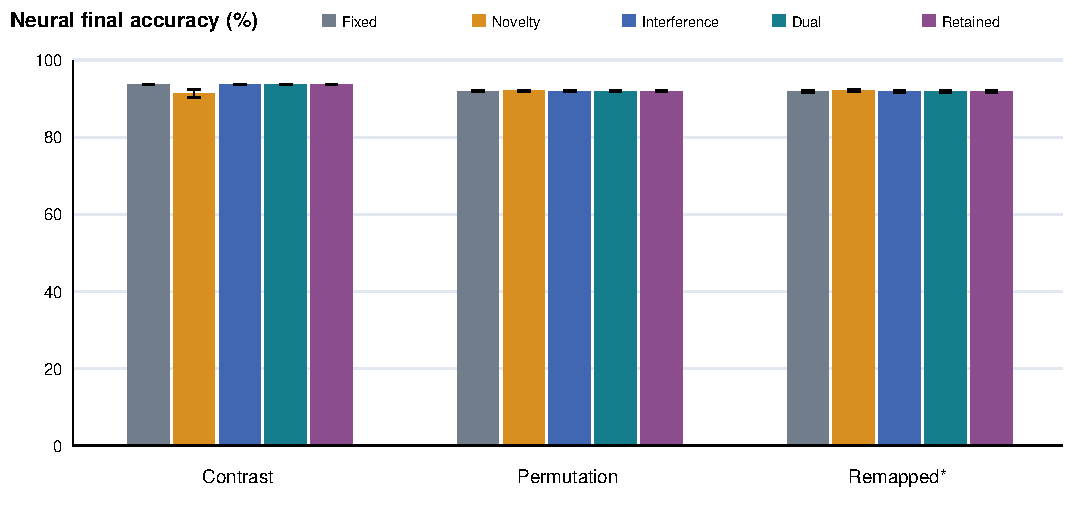
\includegraphics[width=\textwidth]{neural_accuracy.pdf}
\caption{MNIST-derived results. Bars show five-seed means and error bars show sample SD. Target remapping is an additional exploratory stress, not the ordinary digit-recognition task. Fixed, Interference, Dual and Retained overlap because their predictions match in every seed.}
\label{fig:neural_accuracy}\end{figure*}

\subsection{Neural permutation: small accuracy loss with lower allocation}
Novelty averages \(2.80\pm0.45\) networks at \(92.00\pm0.31\%\). Dual retains one at \(91.95\pm0.26\%\). Their accuracy difference is -0.047 points, with interval [-0.192,0.051]. The lower endpoint is above the neural protocol's descriptive -1-point tolerance, while allocation decreases by 1.8 networks. That satisfies the specified descriptive criterion for this stream, not a general noninferiority claim.

One Novelty seed creates only two networks. With multiple old anchors nearly equally distant from a new permuted context, the candidate can change during the three-window streak. Gallery admission can again precede allocation. Input novelty and candidate persistence therefore interact even in the nominal novelty-only baseline. Its expert count is an observed outcome rather than an assumed one-per-domain upper bound.

Fixed capacity again matches Dual. A shared two-hidden-layer network can learn multiple distinct pixel arrangements with replay at this scale. The input transformations do not establish that its representational capacity is inadequate. Slightly greater Dual forgetting, 0.40 points versus 0.07, also shows why a near-matching final mean should not conceal all retention differences.

\subsection{Exploratory target-remapping stress}
After adding incompatible domain-specific label mappings, Novelty reaches \(92.02\pm0.35\%\) with \(2.80\pm0.45\) networks. Dual reaches \(91.77\pm0.30\%\) using one. The paired difference is -0.248 points, with interval [-0.393,-0.079]. This is a small but consistently unfavorable observed difference; it should not be described as equal accuracy. It remains within the specified one-point descriptive tolerance, which is a different statement.

The fixed network still matches Dual. Distinct pixel permutations make the remapped domains distinguishable from input, and the network can represent conditional mappings. Label incompatibility alone therefore does not force growth. The stress does not demonstrate a regime where extra neural capacity is required. Because it was added after the original neural experiment started, it supplies exploratory evidence and is kept separate from the 50 initial runs.

\subsection{Retained evidence changes eligibility without improving these runs}
Retained marks two newly admitted contexts for 30 subsequent windows in each seed: 300 retained windows per stream over five seeds. It increases true gate windows from 3 to 12 on contrast, 0 to 8 on permutation, and 1 to 5 on remapping. However, none forms three consecutive conflicts with the same candidate after warm-up and cooldown. Retained therefore allocates no additional expert and exactly matches Dual predictions.

Interference exceeds 0.2 in 70 contrast, 44 permutation and 40 remapped windows across the five seeds. Isolated opposition exists, but it does not persist sufficiently for these controllers. The unit sequence establishes that Retained can change a delayed decision; the real-image experiment does not establish an accuracy or robustness gain from that change. A more difficult, independently selected setting would be needed to test that benefit rather than lowering the threshold after inspecting these test logs.

\subsection{Resource consequences depend on expert scale}
Synthetic experts occupy 24 weight-array bytes. In benign data, Dual's 1.9-expert reduction saves only 45.6 retained bytes, approximately 0.31\%; replay dominates. Joint control processes about 33\% more gradient examples. This is a weak resource trade-off despite fewer experts.

Each neural expert occupies 437,544 bytes. On contrast, Novelty retains 2.804 MiB versus 1.969 for Dual, a 29.8\% reduction. On permutation and remapping the corresponding means are 2.720 and 1.969 MiB, about 27.6\%. Replay alone occupies 1,617,920 bytes. These are meaningful retained-array differences at this model scale, but are not process-memory, peak-training or GPU-memory measurements.

Dual processes 294,780 gradient examples per neural run versus 235,904 for Novelty, approximately 25.0\% more. The fixed model achieves the same predictions and recorded storage as Dual while avoiding those diagnostic gradients. Thus larger experts change the magnitude of savings relative to Novelty without establishing that the joint controller is the most efficient available policy. CPU times are small and hardware-sensitive; no reliable deployment speedup is claimed.

\section{Discussion and Limitations}
\subsection{What the combined evidence supports}
The synthetic and neural studies address different parts of the question. Logistic experts make incompatible rules difficult to share and expose under-allocation. Neural experts learn representations that can accommodate several transformed image domains. A rule that allocates fewer experts can mean useful sharing in one setting and missed learning in another. The interpretation must therefore include accuracy, forgetting, representational flexibility and the fixed baseline.

The joint hypothesis receives conditional support relative to novelty-only allocation. It suppresses growth under compatible synthetic shifts and all three tested neural streams. However, it underperforms on conflicting synthetic rules and does not outperform fixed neural capacity. The neural evidence is therefore stronger for questioning novelty-driven allocation than for recommending interference as an indispensable second signal.

The retained variant tests a concrete information-management idea. Routing can recognize a context while the allocation controller still needs evidence that adaptation remains unresolved. Retaining a bounded flag separates those notions temporarily. Its neural outcomes are identical to Dual because persistent conflict is absent, so we do not claim that the proposed change fixes the empirical accuracy problem. A possible mechanism and a beneficial intervention are distinct research claims.

\subsection{Limits of representation and routing}
The synthetic context/predictor split is deliberately supplied. In neural runs the artificial split is removed, but routing still uses fixed raw pixels. Pixel permutations and intensity changes have accessible marginal signatures. Neither study tests a learned context embedding, overlapping natural domains, gradual drift, imbalanced open-world streams or mixed-domain batches. Prototype averaging can also be sensitive to class composition within a batch.

A nearest-prototype router may fail even if experts have sufficient capacity. Allocating an expert at recognized context reassigns an anchor and can make previous experts unreachable. Stored count therefore differs from usable inference capacity. A complete lifecycle would need retirement, reuse and routing-repair mechanisms; those remain outside the implemented scope. Opposite rules with indistinguishable input require additional information, rather than simply another slot.

The MLP extension is genuine pixel-based neural learning, but remains small and data-limited. MNIST is a single handwritten-digit dataset; constructed transformations do not establish performance on natural images, CIFAR-100, ImageNet-R, DomainNet, CLIP or low-rank adapters. We have neither reproduced modern expansion systems nor compared their published benchmark scores with these results. More modern architectures would change optimization, gradient geometry, representation drift and resource ratios.

\subsection{Selection, uncertainty and measurement}
The original synthetic ablations follow observed failures. The neural two-stream protocol is specified before its official testing, but was itself designed after those synthetic observations. The added remapping stress is explicitly exploratory. All neural settings use the same MNIST test images under transformations, so they do not constitute three independent dataset confirmations. Five seeds are a small basis for uncertainty, and resampling cannot remove shared-dataset dependence.

The one-point neural tolerance is a declared descriptive decision rule, not a statistical proof of preserved accuracy or a criterion selected for the old synthetic findings. Bootstrap intervals lack multiplicity correction. A future confirmatory study should specify its acceptable loss, primary comparison, scenario selection and power before independent testing. Reporting the remapped loss as zero would be inaccurate even though it falls inside the tolerance.

Endpoint forgetting misses short-lived failures and does not measure forward transfer. Final averages can hide domain differences and task-dependent routing errors. Gradient-example counts omit the arithmetic and memory traffic of routing, while retained arrays omit interpreter overhead and temporary peaks. CPU timing uses this machine's execution environment and should not be generalized to deployment latency.

\subsection{Next experiments}
The most direct next step is a factorial study of trigger persistence and prototype-admission delay, including an explicit no-retention control and several evidence lifetimes. It should measure when an unresolved flag is informative rather than simply how often it causes expansion. A benchmark with independently selected stronger interference would test whether a retained gate rescues useful learning, while avoiding a post-test search for favorable thresholds.

Other controls should vary expert capacity, replay size, context overlap and task order. A matched-compute comparison should charge the extra diagnostic gradients. Direct historical-loss probes or norm-aware conflict scores may be more stable near convergence than cosine alone. An oracle routing diagnostic could separate a bad allocation decision from failure to select an existing specialist, provided its task information is clearly excluded from the actual learner.

A staged real-data extension should first compare learned fixed embeddings with raw pixels, then a small convolutional expert on a harder image dataset under the same access restrictions. Only after establishing reliable accuracy--resource behavior would frozen backbones and lightweight adapters be justified. Such an extension should preserve full source and logs, retain a fixed-capacity baseline and report adverse streams alongside favorable ones.

\balance
\section{Conclusion and Future Work}
This project studies when a continual learner should allocate an expert. Novelty and historical gradient interference provide complementary local evidence, but their usefulness depends on evolving routing state and the capacity already available. A bounded synthetic study with ten matched seeds shows selective sharing under benign changes and unreliable specialization under conflicting rules. Prototype admission can remove novelty before a joint persistence condition completes.

The neural extension trains 109,386-parameter experts from real MNIST pixels and evaluates 75 runs over two initial streams and an additional exploratory remapping stress. Relative to novelty-only allocation, joint control uses one network with similar or higher final accuracy and about 28--30\% less recorded storage. It also computes about 25\% more gradient examples. Fixed capacity exactly matches its predictions, so these outcomes do not establish a need for the adaptive controller.

A bounded retained-evidence revision increases eligible gate windows but produces no additional allocation or accuracy improvement. This negative intervention result constrains the proposed remedy: evidence persistence cannot help when conflict does not itself persist. Future work should isolate trigger and gallery timing, test stronger independently chosen interference, evaluate learned routing and charge computation alongside storage. The present evidence supports transparent allocation analysis and a small neural extension, not a broadly validated expert lifecycle or large-model method.

\section*{Author Responsibilities and AI Assistance}
Mingqi Li reviewed the methodology, verified the code and data-isolation checks, reproduced the experiments, and revised the Methodology and Experimental Protocol sections. Kaiyue Zhang verified the literature and citations, independently checked and interpreted the reported results, analyzed failure cases and resource trade-offs, and revised the Related Work, Results, Discussion and Conclusion sections. Both authors refined the research questions, Introduction and Abstract, cross-reviewed the methods and findings, and completed a final reading and verification of the manuscript. Presentation preparation and rehearsal remain shared responsibilities.

Generative-AI assistance was used for implementation, analysis and draft preparation. Both authors critically reviewed, revised and verified the AI-assisted material and accept responsibility for the accuracy and integrity of the final submission.

\clearpage
\begin{thebibliography}{11}
\bibitem{pnn} A. A. Rusu \emph{et al.}, ``Progressive neural networks'', arXiv:1606.04671, 2016. [Online]. Available: \url{https://arxiv.org/abs/1606.04671}
\bibitem{expertgate} R. Aljundi, P. Chakravarty, and T. Tuytelaars, ``Expert Gate: Lifelong learning with a network of experts'', in Proc. CVPR, 2017, pp. 3366--3375. [Online]. Available: \url{https://arxiv.org/abs/1611.06194}
\bibitem{den} J. Yoon, E. Yang, J. Lee, and S. J. Hwang, ``Lifelong learning with dynamically expandable networks'', in Proc. ICLR, 2018. [Online]. Available: \url{https://arxiv.org/abs/1708.01547}
\bibitem{l2g} X. Li, Y. Zhou, T. Wu, R. Socher, and C. Xiong, ``Learn to Grow: A continual structure learning framework for overcoming catastrophic forgetting'', in Proc. ICML, PMLR 97, 2019, pp. 3925--3934. [Online]. Available: \url{https://proceedings.mlr.press/v97/li19m.html}
\bibitem{gem} D. Lopez-Paz and M. Ranzato, ``Gradient episodic memory for continual learning'', in Advances in Neural Information Processing Systems, vol. 30, 2017. [Online]. Available: \url{https://arxiv.org/abs/1706.08840}
\bibitem{agem} A. Chaudhry, M. Ranzato, M. Rohrbach, and M. Elhoseiny, ``Efficient lifelong learning with A-GEM'', in Proc. ICLR, 2019. [Online]. Available: \url{https://arxiv.org/abs/1812.00420}
\bibitem{der} S. Yan, J. Xie, and X. He, ``DER: Dynamically expandable representation for class incremental learning'', in Proc. CVPR, 2021, pp. 3014--3023. [Online]. Available: \url{https://arxiv.org/abs/2103.16788}
\bibitem{foster} F.-Y. Wang, D.-W. Zhou, H.-J. Ye, and D.-C. Zhan, ``FOSTER: Feature boosting and compression for class-incremental learning'', in Proc. ECCV, 2022, pp. 398--414. [Online]. Available: \url{https://arxiv.org/abs/2204.04662}
\bibitem{memo} D.-W. Zhou, Q.-W. Wang, H.-J. Ye, and D.-C. Zhan, ``A model or 603 exemplars: Towards memory-efficient class-incremental learning'', in Proc. ICLR, 2023. [Online]. Available: \url{https://arxiv.org/abs/2205.13218}
\bibitem{moeadapters} J. Yu \emph{et al.}, ``Boosting continual learning of vision-language models via Mixture-of-Experts adapters'', in Proc. CVPR, 2024, pp. 23219--23230. [Online]. Available: \url{https://arxiv.org/abs/2403.11549}
\bibitem{mnist} Y. LeCun, C. Cortes, and C. J. C. Burges, ``MNIST handwritten digit database,'' 2010. [Online]. Available: \url{https://www.tensorflow.org/datasets/catalog/mnist}
\end{thebibliography}



\end{document}



